\section{Overview} \label{sec:overview}

%%\subsection{\xxx} 

\begin{figure}[tb]
    \centering
\begin{verbatim}
Main Algorithm:
    Input: Program to run + buggy test case
        + (optional) similar baseline test case
    Output: Sequence of actions or UI events which
        trigger the performance problem, and trace
        of execution across event handlers

1. Run program under \xxx, trigger baseline case (if possible)
    and then buggy test case
2. Set heuristics = { default heuristics }
3. Compute graph using current heuristics with
    Algorithm ComputeControlFlowGraph
4.a. If the buggy case is busy executing code (livelock):
        run backward traversal of edges until UI event found
4.b. Else, given a hanging node N_1, use Algorithm
    FindSimilarNode to obtain an equivalent
    in the baseline test case, N_0 \leftarrow FindSimilarNode(N_1)
    5.a. Compare nodes N_0 and N_1, and automatically
        diff the two cases, moving through history semi-automatically
        with user input until useful UI events are found
        [Algorithm AssistedGraphDiff]
    5.b. If new heuristics were added, go to step 3.
6. Return set of UI events found
\end{verbatim}
    \caption{Main \xxx algorithm.}
    \label{fig:alg-main}
\end{figure}

\subsection{\xxx Work Flow}

\begin{figure*}[tb]
    \centering
	%\documentclass{article}
%\usepackage{tikz}
%\usepackage{tikzpeople}
%\usetikzlibrary{shapes, shapes.misc}
%\usetikzlibrary{arrows, arrows.meta, decorations.markings}
%\usetikzlibrary{patterns}

%\usetikzlibrary{calc,backgrounds}
%\usepackage[active,tightpage]{preview}
% taken from manual
\makeatletter
\pgfdeclareshape{document}{
\inheritsavedanchors[from=rectangle] % this is nearly a rectangle
\inheritanchorborder[from=rectangle]
\inheritanchor[from=rectangle]{center}
\inheritanchor[from=rectangle]{north}
\inheritanchor[from=rectangle]{south}
\inheritanchor[from=rectangle]{west}
\inheritanchor[from=rectangle]{east}
% ... and possibly more
\backgroundpath{% this is new
% store lower right in xa/ya and upper right in xb/yb
\southwest \pgf@xa=\pgf@x \pgf@ya=\pgf@y
\northeast \pgf@xb=\pgf@x \pgf@yb=\pgf@y
% compute corner of ‘‘flipped page’’
\pgf@xc=\pgf@xb \advance\pgf@xc by-10pt % this should be a parameter
\pgf@yc=\pgf@yb \advance\pgf@yc by-10pt
% construct main path
\pgfpathmoveto{\pgfpoint{\pgf@xa}{\pgf@ya}}
\pgfpathlineto{\pgfpoint{\pgf@xa}{\pgf@yb}}
\pgfpathlineto{\pgfpoint{\pgf@xc}{\pgf@yb}}
\pgfpathlineto{\pgfpoint{\pgf@xb}{\pgf@yc}}
\pgfpathlineto{\pgfpoint{\pgf@xb}{\pgf@ya}}
\pgfpathclose
% add little corner
\pgfpathmoveto{\pgfpoint{\pgf@xc}{\pgf@yb}}
\pgfpathlineto{\pgfpoint{\pgf@xc}{\pgf@yc}}
\pgfpathlineto{\pgfpoint{\pgf@xb}{\pgf@yc}}
\pgfpathlineto{\pgfpoint{\pgf@xc}{\pgf@yc}}
}
}
\makeatother

%\begin{document}
\begin{center}

%%\resizebox{0.8\textwidth}{0.4\textwidth}{%
\resizebox{0.48\textwidth}{!}{%
\begin{tikzpicture}[>=latex]

% We need layers to draw the block diagram
\pgfdeclarelayer{background}
\pgfdeclarelayer{foreground}
\pgfsetlayers{background,main,foreground}

\tikzstyle{every node}=[font=\Large]
\tikzstyle{apps} = [draw, very thick, minimum height=3em, minimum width=5em, fill=white, rectangle, font={\sffamily\bfseries}]
\tikzstyle{systemComp} = [draw, very thick, minimum height=3em, minimum width=15.1em, fill=white, rectangle, font={\sffamily\bfseries}]
\tikzstyle{actionLabel} = [draw, pattern=north west lines, pattern color = red!20, ellipse, minimum width = 15em, minimum height= 5em]%shape aspect=3, minimum size=30, diamond]

\tikzstyle{doc} = [draw, thick, align=left, color=black, shape=document, minimum width=18em, minimum height=12em, shape=document, inner sep=2ex]
\tikzstyle{commanddoc} = [draw, thick, align=left, color=black, shape=document, minimum width=5em, minimum height=8em, shape=document, inner sep=2ex]
\tikzstyle{debuglogdoc} = [draw, thick, align=left, color=black, shape=document, minimum width=8em, minimum height=6em, shape=document, inner sep=2ex]
\tikzstyle{mininode} = [draw, rectangle, minimum height=1em, minimum width=1em]

\tikzstyle{prearrow} = [-, thick, line width=1em] %double distance = 1.2em, shorten >=-0.2em]
\tikzstyle{vecarrow} = [->, thick, line width=1em] %double distance = 1.2em, shorten >=-0.2em]
%\tikzstyle{vecarrow} = [thick, decoration={markings, mark=at position
   %1 with {\arrow[xshift=1.2em, scale=0.6] {triangle 90}}},
   %1 with {\arrow[xshift=1.5em]{Straight Barb[length=2pt 0.7]}}},
   %double distance=1.2em,
   %postaction= {decorate}]

%draw MacOS components
\node [apps, name=software1] at (0, 0) {chromium};
\node [apps, name=software2, right of=software1, node distance=5em] {daemon1};
\node [apps, name=software3, right of=software2, minimum width=5.2em, node distance=5em] {daemon2};
\node [systemComp, name=libs, below left = 0em and -10.21em of software2] {libs};
\node [systemComp, name=kernel, below of=libs, node distance=3em] {kernel};
\node (MacOS) [below of = kernel, minimum width=15em, node distance = 3em] {MacOS};

% draw Tracing Event log
\node (TracingEventLog) [minimum height=3em, minimum width=20em, right of=software3, node distance=22em] {TracingEventLog};
\node [doc, below of=TracingEventLog, name=log, node distance=4em] {\#timestamp, event\_type, att1, att2...\\30.4 Mach\_message 0x4ea20 0x3...\\31.7 Mach\_message 0x4ea20 0x3...\\33.2 Wake\_up 0xea45 0x16...};

%draw arrow from MacOS to Tracing Event log
%\draw[vecarrow, shorten >= -0.05em] (libs.east)+(0.5, 0) -- (log.west);%(TracingEventLog.west);
\draw[vecarrow] (libs.east)+(0.5, -0.35) -- (log.west);%(TracingEventLog.west);

%draw Arrow for Constructing Graph
\node [actionLabel, below of=log, node distance=9.5em, name=action1] {Construct Graph};
\draw [prearrow] (log.south) -- (action1.north);

%draw Dependency Graph
\node (DependencyGraph) [minimum height=3em, minimum width=20em, below of=action1, node distance=8em] {Dependency Graph};
\node [mininode, below of=DependencyGraph] (1c3) {};
\node [mininode, left of=1c3, node distance=2em] (1c2) {};
\node [mininode, below of=1c2, node distance=2em] (2c2) {};
\node [mininode, left of=2c2, node distance=2em] (2c1) {};
\node [mininode, left of=2c1, node distance=2em] (2c0) {};
\node [mininode, right of=2c2, node distance=2em] (2c3) {};
\node [mininode, right of=2c3, node distance=2em] (2c4) {};
\node [mininode, below of=2c0, node distance=2em] (3c0) {};
\node [mininode, right of=3c0, node distance=2em] (3c1) {};
\node [mininode, right of=3c0, node distance=6em] (3c2) {};
\node [mininode, below of=3c0, node distance=2em] (4c0) {};
\draw [->] (1c2.south) -- (2c0.north);
\node (DGendline)[minimum height=1em, minimum width=20em, below of=DependencyGraph, node distance=10em]{};

%\draw [vecarrow, shorten <=-0.2em, shorten >= 0.1em] (action1.south) -- (DependencyGraph.north);
\draw [vecarrow] (action1.south) -- (DependencyGraph.north);

%draw interactive Debugging part
\node [commanddoc, left of=DependencyGraph, node distance=18em](command){Debugging command\\search\_node\\check\_node\\lldb:br\\lldb:si};
\node[alice, minimum size=3em, left of=command, node distance=8em](user) {};
\node [debuglogdoc, left of=user, node distance=8em](debuglog){Debugging log:\\path: ...\\node\_id: ...\\execution\_list:\\  movq \%rax, \%rcx \\...};%\\  movq \$1, \%rbx\\  ...};
\node [actionLabel, below of=user, node distance=8em, name=action2] {Interactive Debugging};
\draw [->] (user.east) to [out=330,in=60] (action2.north east);
\draw [->] (action2.north west) to [out=120,in=210] (user.west);
\draw [->] (user.north)+(0, 0.1) to (libs.south);
\draw [prearrow](DGendline.north west) + (0, 0.5) -- (action2.east);
%\draw [prearrow, -, shorten >= -1.8em](DGendline.north west) + (0, 0.5) -- (action2.east);
%\node (result) [draw, rectangle, align=left, minimum height=2em, minimum width=20em, below of = action2, node distance=6em] {RootCause:\\UI thread blocking in Chromium because of\\wating for message from Render thread};
%\draw [vecarrow, shorten <= -0.2em] (action2.south) -- (result.north);

\node (result) [draw, rectangle, align=left, minimum height=20em, minimum width=9em, text width=8em, left of=debuglog, node distance=12em] {RootCause:\\UI thread of Chromium blocks due to wating for message from render thread};
\node (alignresult)[left of=action2, node distance=16em]{};
%\draw [vecarrow, shorten <= -1.8em] (action2.west) -- (alignresult.east);
\draw [vecarrow] (action2.west) -- (alignresult.east);

\begin{pgfonlayer}{background}
%%draw background rectangle for macos, graph and debugging log
\path (software1.west |- software3.north)+(-0.5, 0.5) node (a) {};
\path (MacOS.south east)+(0.5, -0.5) node (b) {};
\path[fill=yellow!20,rounded corners, draw=black!50, dashed] (a) rectangle (b);
%%draw backgroud for dependancy graph
\path (DependencyGraph.west |- DependencyGraph.north) node (a) {};
\path (DGendline.south east) node (b){};
\path[fill=yellow!20,rounded corners, draw=black!50, dashed] (a) rectangle (b);
%%draw background for interactive debugging
%\path (IDbeginline.west |- IDbeginline.north) node (a) {};
%\path (IDendline.south east) node (b) {};
%\path[fill=yellow!20,rounded corners, draw=black!50, dashed] (a) rectangle (b);

\end{pgfonlayer}
\end{tikzpicture}
}
\end{center}
%\end{document}

    \caption{\xxx Work Flow}
    \label{fig:argus-overview}
\end{figure*}

Figure~\ref{fig:argus-overview} shows \xxx's work flow, which consists of two
phases.  A user runs command ``\vv{\xxx start}'' to enter the system-wide
tracing phase, within which \xxx logs events including system calls,
inter-process communications (IPCs), and waits and wake-ups from all
applications and daemons.  Occasionally based on user configurations, it logs
data flag accesses leveraging hardware watch-point registers.  Each log entry
includes a timestamp, the event type, key attributes of the event, and a
lightweight call stack obtained by unwinding the stack pointer.  \xxx
implements tracing by instrumenting core system libraries and a small portion
of the operating system.  The performance impact of this system-wide tracing is
low because the logged events themselves are often expensive and require
user-kernel crossings, masking the overhead of tracing.

Whenever a user detects a performance issue such as a spinning cursor, she runs
``\vv{\xxx debug}'' to enter the interactive diagnosis phase.  \xxx initializes
this phase by constructing a causal graph from all logged events up to
user-specified duration.  Rather than requiring a precise application-specific
user-written schema, \xxx leverages a simple system-wide schema we created to
construct approximate graphs (\S\ref{subsec:graph}), and relies on interactive
user insights for diagnosis (\S\ref{subsec:debug}).

\subsection{Constructing Event Graphs} \label{subsec:graph}
\section{Argus Graph Computing}\label{sec:graphcomputing}

\subsection{Event Graph}\label{subsec:eventgraph}
%%Main point for the subsection: \xxx computes a dependency graph to assist
%%debugging. It is a useful graph to figure out relationships across thread
%%boundary and timing boundary 
%%
%%\begin{itemize}
%%\item What the graph is?
%%
%%	\begin{itemize}
%%	\item Paragraph1: high level description of dependency graph.
%%
%%\xxx constructs dependency graphs with the events from tracing logs. Tracing
%%logs contains sequence of events per thread. Each event stands for an execution
%%step in the thread. They are grouped into nodes and IPCs, asynchronouns calls
%%and thread wakeups serve as edges; some edges can be inside a single thread.
%%
%%	\item Paragraph2: detail about the graph.
%%
%%Events can be classed into three categories: semantic, connection, boundary
%%Graph nodes consist of a list of execution events and edges are generated with
%%event pairs.
%%
%%	\end{itemize}
%%
%%\item Why the graph is userful?
%%The graph bares the causility path of a user input and thus is helpful in
%%debugging complicated performance bugs, which involve mutilple processes and
%%threads.
%%\end{itemize}

\xxx constructs dependency graphs with the events from tracing logs. Tracing
logs contain sequence of events per thread. Each event stands for an execution
step in a thread. They are grouped into nodes and IPCs, asynchronouns calls
and thread wakeups serve as edges; some edges can be inside a single thread.

The events traced in \xxx are carefully selected for three main purposes:
preserve semantics for the node, indentify node boundary inside a thread, and
provide connections between nodes. We classify them into three categories:
semantics events, boundary events and connection events, as listed in
Table~\ref{table:event_types}.

\begin{table}[h]
  \centering
  \begin{tabularx}{\columnwidth}{|X|X|}
  	\hline
    \textbf{Categories} & \textbf{Event types}\\
	\hline
	\hline
    {\bf Semantics Events} & System\_call\\
    provide hints for user & Back\_trace\\					   
	interactive debugging  & NSApp\_event\\
    \hline
    {\bf Boundary Events} & Interrupts\\
	construct nodes & Sharetime\_maintenance\\
	& Wait\\
	& Dispatch\_invoke\\
    & Runloop\_invoke\\
	& Mach\_message\\
    \hline
	{\bf Connection Events} & Wake\_up\\
    add edges & Mach\_message\\
    & Dispatch\_enqueue\\
    & Runloop\_submit\\
	& Share\_flag\_write\\
	& Share\_flag\_read\\
    \hline
  \end{tabularx}
  \caption{Event Type Categories. }
  \label{table:event_types}
\end{table}

Given the prevalent of multi-threading and multi-processing programs, bugs are
much more complicated. The long opening bugs are usually have several threads
involve, even across process boundaries. As an example, the always timeout on
particular synchronization primitive in one thread usually need to trace back to
find the other thread that was responsible for signal on the primitive. Compared
to the existing debugging tools like lldb and spindump, the dependency graph is
useful in that 1) it provides thread relationships all over the system across
processes boundary and timing boundary and 2) it records execution history for
an input event before users capture hangs with their eyes.

\subsection{Inherent Inaccuracy}\label{subsec:inherentinaccuracy}
%%main point: the inaccuracy of causality graph
%%\begin{itemize}
%% 	\item Paragraph1: describe the inaccuracy with general idea, define over
%%connection and under connection
%%
%%	
%%	\item Paragraph2: over connection patterns
%%
%%Over connections occur if intra-thread boundaries are missing from batch
%%processing programming paradigms. (dispatch\_mig\_service, runloop)
%%
%%	\item Paragraph3: under connection patterns
%%
%%Data dependencies inter/intra threads are usually hard to fully exploit in the
%%initial pass of graph computing. (shared flags in Object, data dependency for
%%delay work intra-thread)
%%
%%\end{itemize}

However, to construct an accurate and complete dependency graph is difficult,
if not impossible. The graph is inherently inaccurate. That one thread wakes
up the other thread does not always stand for a causility between them. In
implementation, \xxx filters out some of the definitive noise in the following
types.

%%We identify the purpose of wake-up and add huristics to filter out the false edges.

\begin{itemize}

\item interrupt processing and kernel sharetime maintanance that take over
current thread context.

\item timer expiration in the kernel which clears up all the waiting threads on
an event source.

\end{itemize}

In addition to the known definitive noise, there exist false connections and
miss data dependencies based on our experience while building dependency graph
with traditional causality tracing. We define them as over connection and under
connection respectively.

Over connections occur if intra-thread boundaries are missing from batch
processing programming paradigms. (dispatch\_mig\_service, runloop)

\para{Dispatch message batching}
The message dispatch service dequeues messages from many processes and staggers
processing of the messages. This creates false dependencies between each message
in the dispatch queue. As illustrated in the following code snipped from the
\vv{fontd} daemon, function \vv{dispatch\_execute} is installed as a callback to
a dispatch queue. It subsequently calls \vv{dispatch\_mig\_server()} which runs
the typical server loop and handles many messages.

To avoid incorrectly linking many irrelevant processes through such batching
processing patterns, \xxx adopts the aforementioned heuristics to split an
execution segment when it observes that the segment sends out messages to two
distinct processes. This pattern does pose a challenge for automated causal
tracing tools that assume that the entire execution of a callback function is
on behalf of one request. The code shown uses a dispatch-queue callback, but
inside the callback, it does work on behalf of many different requests. Any
application or daemon can implement its own server loop this way, which makes it
fundamentally difficult to automatically infer event handling boundaries.

{\footnotesize \begin{verbatim}
Worker thread in fontd daemon:
dispatch_async(block)

Main thread in fontd daemon:
block = dispatch_queue.dequeue()
dispatch_execute(block)
  dispatch_mig_server()

dispatch_msg_server()
  for(;;)
    mach_msg(send_reply, recev_request)
    call_back()
    set_reply()
\end{verbatim}
}

\para{Runloop callbacks batch processing}
As is common in event driven programming, many methods can post a callback and
MacOS uses runloop as a common idiom to process callbacks. As shown in the
following step-by-step description of the MacOS runloop, an iteration of the
runloop does 10 different stages of processing, each of which may do work on
behalf of completely irrelevant requests. Since there are no obvious events
(\eg, a wait operation) to split the execution, \xxx uses instrumentation to
add beginning and ending points for MacOS runloops. In general, any application
or daemon can create its own version of the runloop, posing challenges for
automated inference of event processing boundaries.

% // another thread installs cb
% performSelector:onThread:withObject:waitUntilDone;

{\footnotesize \begin{verbatim}
Run loop sequence of events //developer.apple.com
1-3.Notify observers
4.Fire any non-port-based input sources
5.If a port-based input source is ready and waiting to fire,
    process the event immediately. Go to step 9.
6.Notify observers that the thread is about to sleep.
7.Put the thread to sleep until:
    //one of the following events occurs
    An event arrives for a port-based input source.
    A timer fires.
    The timeout value set for the run loop expires.
    The run loop is explicitly woken up.
8.Notify observers that the thread just woke up.
9.Process the pending event.
  If a user-defined timer fired,
    process the timer event
    restart the loop.
    Go to step 2.
  If an input source fired
    deliver the event.
  If the run loop was explicitly woken up, but not timed out,
    restart the loop. Go to step 2.
10.Notify observers that the run loop has exited.

\end{verbatim}
}

\para{Batching and data dependency in event processing}
The WindowServer MacOS system daemon contains an event loop which waits on
Mach messages. Conceptually, it processes a series of independent events from
different processes. However, to presumably save on kernel boundary crossings,
it uses a single system call to receive data and send data for an unrelated
event. This batch processing artificially makes many events appear dependent,
and we split the execution segments to maintain the independence of the events.

This case also illustrates a causal linkage caused by data dependency within
one thread. As the code shows, WindowServer saves the reply message in variable
\vv{\_gOutMsg} inside function \vv{CGXPostReplyMessage}. When it calls
\vv{CGXRunOneServicePass}, it sends out \vv{\_gOutMsg} if there is any pending
message. This data dependency needs to be captured in order to establish a
causal link between the handling of the previous request and the send of the
reply. Interestingly, it is an example of a data dependency within the same
thread. \xxx uses watch point registers to capture events on these data flags
and establish causal links between them.

{\footnotesize \begin{verbatim}
while() {
  CGXPostReplyMessage(msg) {
  // send _gOutMsg if it hasn't been sent
    push_out_message(_gOutMsg)
    _gOutMsg = msg
    _gOutMessagePending = 1
  }
  CGXRunOneServicePass() {
    if (_gOutMessagePending)
      mach_msg_overwrite(MSG_SEND | MSG_RECV, _gOutMsg)
    else
      mach_msg(MSG_RECV)
    ... // process received message
  }
}
\end{verbatim}
}

Under connections are result from particular programing paradigms and data
dependencies. Data dependencies inter/intra threads are usually hard to fully
exploit in the initial pass of graph computing. (shared flags in Object, data
dependency for delay work intra-thread)

\para{CoreAnimation shared flags}
A worker thread can set a field \vv{need\_display} inside a CoreAnimation object
whenever the object needs to be repainted. The main thread iterates over all
animation objects and reads this flag, rendering any such object.

This shared-memory communication creates a dependency between the main thread
and the worker so accesses to these field flags need to be tracked. However,
since each object has such a field flag, \xxx cannot afford to monitor each
using a watch point register. Instead, it uses instrumentation to modify the
CoreAnimation library to trace events on these flags.

{\footnotesize \begin{verbatim}
Worker thread that needs to update UI:
ObjCoreAnimation->need_display = 1

Main thread: 
traverse all CoreAnimationobjects
if (obj->need_display == 1)
  render(obj)

\end{verbatim}
}

\para{Spinning cursor shared flag}
Whenever the system determines that the main thread has hung for a certain
period, and the spinning beach ball should be displayed, a shared-memory flag
is set. Access to this flag is controlled via a lock, i.e. the lock is used for
mutual exclusion, and does not imply a happens before relationship. Thus, \xxx
captures accesses to these flags using watch-point registers to add causal edges
correctly.

{\footnotesize \begin{verbatim}
NSEvent thread:
CGEventCreateNextEvent() {
  if (sCGEventIsMainThreadSpinning == 0x0)
     if (sCGEventIsDispatchToMainThread == 0x1)
       CFRunLoopTimerCreateWithHandler{
         if (sCGEventIsDispatchToMainThread == 0x1)
           sCGEventIsMainThreadSpinning = 0x1
           CGSConnectionSetSpinning(0x1);
       }
}

Main thread
Convert1CGEvent(0x1);
if (sCGEventIsMainThreadSpinning == 0x1)
  CGSConnectionSetSpinning(0x0);
  sCGEventIsMainThreadSpinning = 0x0;
  sCGEventIsDispatchedToMainThread = 0x0;
\end{verbatim}
}

In addition, the spurious edge introduced by mutex lock is also a challenge in
debugging. The synchronization on mutex lock reflects one thread wakes up the
other thread. They can depend on each other like producer and comsumer, while
no causality exists in the case of contention for a shared resource. Making the
graph completely sound without user interaction is almost impossible given the
essential attribite of commericial operating system as a grey box.

\subsection{User Interactions}

%%Main point for the subsection: why we need user interaction, what the user can
%%do and how it helps
%% Para1 : why we need user interaction
%% Para2 : what the user can do
%% Para3 : how it helps causality tracing

As we mentioned above, to figure out all the over connections and under
connections before hand is almost impossible. Instead, users can find out the
descrepency on the dependency graph while checking the computing result. For
example, we noticed that two unrelated applications connects to one node in the
graph, which leads to the manifestation of kernel thread batch processing on
timers. Users can gradually inject their knowledge until the graph is reasonable
for following debugging.

Over connections in this kind can be eliminated by adding heuristics to the
process of graph computing. In addition, users can also binary instrument the
image with the APIs provided by \xxx to amending the missing boundaries. On
contrary, if users discover under connections due to missing data dependency,
they can make use of the \xxx's hardware breakpointer tool to monitor the data
and add rules to recompute the graph.

Like other causality tracing approaches, \xxx is a general framework and tested
on limited data set. Allowing user interaction makes the dependency graph more
practical and useful case by case.

\subsection{Graph Computing Algorithm}

In the section, we describe the algorithm \xxx used to generate an event graph.
The algrithm has two main steps: construct nodes with heuristics base on
boundary events, and generate edges from the connection events.

A node is a sequence of events derived from the execution of a task in a thread.
As is shown in Figure ~\ref{fig:alg-graphcomputing}, \xxx checks events per
thread and applies heuristics when a boundary event is encoutered. \xxx provides
5 default heuristics. 4 of them shares the idea of general cuasual tracing, 1
is used to work around unknown programming pargdigms, and more are expected
from users to improve graphs. We discuss them in the following paragraph.

As known noises, event sequences for interrupt processing and kernel
maintainance are removed from threads, as is shown in 1.a. The second heuristics
1.b treats a wait event as an end of node. Wait event usually indicates a thread
switches to other tasks, but it is not always true considering a thread may park
due to low thread priority. One of the examples in MacOS is the pause of worker
threads draining a low priority diapatch queue. Dispatch queues are FIFO queues
to which an application can submit tasks in the form of block objects. Wait
events should not divide the block objects, otherwise it may result in a missing
connection. To save the intergrity of block objects, \xxx GraphComputeAlgorithm
keeps a counter \vv{callout\_level} to mark if the currently checking event is
inside a block object. Only the begin and end of Dispatch\_invoke are served
as the boundary for the node, as is shown in the step 1.c. The hueristics 1.d
is also for a batch processing mechanism. Runloop is an event processing loop
that used to schedule work and coordinate the receipt of incoming events.
The begin and end of the work invocation are served as boundaries. The last
default heuristics 1.e is used to work around the problem that batch processing
programming paragdigms are hard to exploit completely, as listed in previous
subsection ~\ref{subsec:inherentinaccuracy}. \xxx makes use of mach messages
to avoid clustering multiple tasks due to unknown batch processing. It defines
\vv{IPC\_peer\_set} to compute the set of mach message receivers/senders for
every node. For every mach message, the algorithm checks whether its peer
process exists in \vv{IPC\_peer\_set}, and adds the message into the current
node if the condition is true or the set is empty. Otherwise it add a boundary
for current node and begin a new node for the mach\_message event.

Edges connect nodes, both intra-thread and iter-thread, with connection events.
\xxx walks through each connection event types to apply heuritics as follows.
First, the return from a wait operation causally depends on the wake-up
operation. An edge is defined from the wake-up event to the first event after
the wait returns. \xxx also add a weak edges from the wait event to the wake-up
event in 2.a. Mach message is the core of ipc mechanism implemented in kernel,
upon which higher level RPC are built. \xxx connects the sender and receiver
of a mach message. For messages that expect a reply, \xxx also connects the
receiver of the original message and the sender of the reply message in 2.b.
As discussed above, dispatch queue and runloop are popular batch processing
programming paradigms in MacOS, \xxx connects submissions of a task and
executions of the task, which are listed in 2.c and 2.d respectively. Similarly,
\xxx adds edge from a timer armed event to its triggered event in 2.e. Shared
flag can either be traced with binary instrument, such as \vv{need\_display}
flag for CoreAnimation in subsection ~\ref{subsect:inherentinaccuracy}, or with
breakpoint watcher command line tool provided by \xxx. Edges from the flag set
to its read are added as 2.f. Since share variables are hard to completely
exploited, and the causality can be complicated than the writer-reader pattern,
user interaction are expected to remedy event graphs.

Finally, the computing graph is generated and subject to the improvement with
more input heuristics.

\begin{figure}[tb]
\footnotesize\begin{verbatim}
Algorithm ComputeControlFlowGraph:
    Input: Heuristics set + parsed tracing events
    Output: Control flow graph
1. Create nodes per thread:
  set callout_level = 0
  1.a interrupt/kern_maintainance: remove_events
  1.b wait: end of node if callout_level == 0
  1.c if dispatch_callout begin, create a new node
      and increase callout_level
      if dispatch_callout end, complete current node
      and decrease callout_level
  1.d Runloop: divide every callout
  1.e mach_msg: divide IPC with different peers
  1.f Other heuristics added by user from the input set.
2. Add edges for connection events:
  2.a wake_up event and wait event
  	edge(wake_up, first_waken_event)
	weak_edge(wait, wake_up)
  2.b mach message
  	edge(sender, receiver)
    if message needs reply
       edge(receiver, reply_sender)
  2.c dispatch queue events
  	edge(work_enqueue, work_dequeue)
  2.d Runloop work submission
  	edge(work_submit, work_invoke)
  2.e timer events
  	edge(timer_armed, timer_fired)
  2.f shared variable
  	edge(set_variable, read_and_clear_variable)
  2.g Other heuristics added by user from the input set.
3. Return the Graph with Nodes and Edges
\end{verbatim}
    \caption{\xxx Compute Graph algorithm.}
    \label{fig:alg-graphcomputing}
\end{figure}

%%\xxx defines the beginning of an execution segment as one of the following
%%three types of events (1) the beginning of a thread, (2) the event from a wait
%%operation such as \vv{pthread\_cond\_wait()} or \vv{mach\_msg\_receive()}, and
%%(3) the first logged event of a thread because tracing may start mid execution.
%%It similarly defines the end of an execution segment as (1) the exit of a
%%thread, (2) the call to a wait operation, and (3) the last logged event of a
%%thread.
%%
%%\xxx defines the edges as follows.  First, the return from a wait operation
%%causally depends on the wake-up operation.  Since an application or its
%%libraries may define custom synchronization primitives, \xxx traces wait and
%%wake-up operations inside the operating system kernel (the
%%\vv{waitq\_assert\_wait64\_locked} and \vv{thread\_unblock} functions in MacOS
%%kernel).  This design decision ensures that \xxx captures a large set of casual
%%edges at the expense of superfluous edges that do not map to causality.  For
%%instance, inside a system call or interrupt handler, the kernel typically
%%checks whether the current process has used up its time slice and, if so, wakes
%%up another process.  \xxx thus explicitly filters out edges due to kernel
%%maintenance (in \vv{interrupt} and \vv{sched\_timeshare\_miantenance\_continue}
%%functions in MacOS) instead of application intent.  Second, the read of a data
%%flag causally depends on the write of the same flag.  Edges of this type are
%%few but critical for diagnosis.  Third, the timer expiration and cancellation
%%events causally depend on the installation of the timer.  Fourth, each
%%execution segment has an incoming edge from the immediately preceding segment
%%in the same thread.  \xxx considers this type of intra-thread edges weaker than
%%inter-thread edges due to the wait between the two segments.  In its analysis,
%%\xxx follows intra-thread edges typically only when it cannot find any
%%inter-thread edges.
%%
%%It is easy for a user to incrementally extend \xxx with custom segment
%%boundaries and edges.  For instance, to handle batch processing, we
%%created a heuristic that splits a segment if it has outgoing edges to two
%%or more different processes (unless the attributes of the corresponding
%%events indicate otherwise).  We also added edges for three data flags and
%%eight custom communication primitives (see \S\ref{subsec:tcp}).

\subsection{Interactive Diagnosis} \label{subsec:debug}

After \xxx builds the event graph, a user can interactively query this graph
for diagnosis.  For instance, consider a spinning cursor in MacOS which
indicates the current application's main thread has not processed any UI events
for over two seconds.  The user can query \xxx to find the ongoing event in the
application's main thread concurrent to the display of the spinning cursor.
Depending on the type of the event, she can proceed in three directions.

First, if the concurrent event is a busy operation that occupies the CPU, she
has found the cause of the spinning because a busy main thread cannot process
UI events.  She can examine the event's lightweight call stack.  If it does not
provide enough details, she can rerun the application and use \xxx's
fine-grained debugging tool to obtain a more complete call stack, the addresses
of the instructions executed, and parameters and return values of call
instructions.  In general, she can increase debugging details for any event,
not just a busy event.

Second, if the concurrent event is a blocking wait, she runs \xxx to locate
another event in the graph that causes the wake-up to arrive late. \xxx does so
using the following idea.  In the normal case, there must be a path of wake-up
edges that leads to the blocking wait, so the main thread starts running again.
In the spinning case, somewhere along the path, a thread's wake-up is missing,
so this thread is the culprit.  Mechanically, \xxx first searches the graph to
find a similar wait that does not cause a spinning cursor.  If there are
multiple nodes similar to the wait, \xxx asks the user to pick one.  It then
slices the graph backwards to find the wake-up path.  If an event has exactly
one inter-thread edge or only an intra-thread edge, it follows the edge.
Otherwise, the event must have two or more inter-thread edges, and \xxx
consults the user to pick one to follow.  Given the path, \xxx examples the
threads in the path one by one, and returns the thread whose wake-up is missing
in the spinning case.

Third, if the concurrent event is a thread yield, it is highly indicative that
the main thread is waiting on a data flag (\eg, ``while(!done)
thread\_switch();'').  To discover a data flag, the user reruns the application
with \xxx to collect instruction traces of the concurrent event in both the
normal and spinning cases and detects where the control flow diverges.  She
then reruns the application with \xxx to collect register values for the basic
blocks before the divergence and uncovers the address of the data flag.  She
then configures \xxx to log accesses to the flag during system-wide tracing.
Finally, she can recursively apply \xxx to further diagnose ``the culprit of
the culprit''. 

Based on our results, the first type of spinning cursor is more common but the
second and third types cause the most harm.  The reason is that the first type
tends to be straightforward to diagnose, so they are fixed quickly.  The second
and third types involve multiple threads, so they are extremely hard to
understand and fix even for the application's own developers.  Therefore, they
remain open for years and ruin many users' experiences.

\subsection{Chromium Spinning Cursor Example}

%   resolve symbol, save to log
%     search for set\_spinning
%     if found,
%       find main thread node at the time of set\_spinning
%     find fontd
%     manually check nodes in each thread immediately after the nodes in the slice (normal abnormal boundary)
%  output is a node, and a HTML dump of node and immediate predecessors and successors
% systems preference          
%  spinning node in UI thread is not waiting
%  so we look for messages, and find the diff

One of the authors experienced first-hand the aforementioned performance issue
in Chromium, an open-source browser engine that powers Google Chrome and,
starting recently, Microsoft Edge~\cite{chromiumurl}.  She tried to type in the
Chromium search box a Chinese word using SCIM, the default Chinese Input Method
Editor that ships with MacOS.  The browser appeared frozen and the spinning
cursor occurs for a few seconds.  Afterwards everything went back to normal.
This issue is reproducible and always ruins her experience, but it is quite
challenging to diagnose because two applications Chromium and SCIM and many
daemons ran and exchanged messages.  This issue was reported by other users for
other non-English input methods, too.

To diagnose this issue with \xxx, the author started system-wide tracing, and
then reproduced the spinning cursor with a Chinese search string typed via SCIM
while the page was loading. It produced normal cases for the very first few
characters, and the browser got blocked with the rest input as spinning cases.
The entire session took roughly five minutes.

She then ran \xxx to construct the event graph.  The graph had 2,749,628
vertexes and 3,606,657 edges, almost fully connected.  It spans across 17
applications; 109 daemons including \vv{fontd}, \vv{mdworker}, \vv{nsurlsessiond}
and helper tools by applications; 126 processes; 679 threads, and 829,287 IPC
messages.  Given the scale of the graph and the diverse communication patterns,
it would be extremely challenging for prior automated causal tracing
tools~\cite{aguilera2003performance, zhang2013panappticon, attariyan2012x,
cohen2004correlating} because they handle a fairly limited set of patterns.
Tools that require manual schema~\cite{barham2004using, reynolds2006pip}, would
be prohibitive because developers would have to provide schema for all involved
applications and daemons.

\begin{figure*}[p]
    \centering
	%%\documentclass{article}
%%\usepackage{tikzpeople}
%%\usepackage{tikz}
%%\usetikzlibrary{shapes, shapes.misc}
%%\usetikzlibrary{arrows, arrows.meta, decorations.markings}
%%\usetikzlibrary{patterns}

%%\begin{document}
\begin{center}
\resizebox{\columnwidth}{!}{%
\begin{tikzpicture}[>=latex]
\tikzstyle{every node}=[font=\Large]
\tikzstyle{app} = [draw, very thick, minimum height=40em, minimum width=20em, fill=white, rectangle, font={\sffamily\bfseries}]
\tikzstyle{actionpoint} = [minimum width = 1em, fill = white]
\tikzstyle{point} = [thick, draw=red, cross out, inner sep = 0pt, minimum width = 0.5em, minimum height =0.5em]
%\tikzset{
%%ext/.pic={
%%\path [fill=white] (-0.2,0)to[bend left](0,0.1)to[bend right](0.2,0.2)to(0.2,0)to[bend left](0,-0.1)to[bend right](-0.2,-0.2)--cycle;
%%\draw (-0.2,0)to[bend left](0,0.1)to[bend right](0.2,0.2) (0.2,0)to[bend left](0,-0.1)to[bend right](-0.2,-0.2);
%%},
%point/.style={
%    thick,
%    draw=red,
%    cross out,
%    inner sep=0pt,
%    minimum width=4pt,
%    minimum height=4pt,
%}}

%draw applications
\node [app, name = browser]{};
\node (browsertag)[minimum width = 20em, above = -2em of browser] {Chromium Browser};
\node (browserend)[minimum width = 20em, below = 38em of browsertag] {};
\node (bt1begin)[minimum width = 8em, below left = 3em and -10em of browsertag]{main thread};
\node (bt1end)[minimum width = 8em, below left = 38em and -10em of browsertag]{};
\node (bt2begin)[minimum width = 8em, below right = 3em and -10em of browsertag]{worker thread};
\node (bt2end)[minimum width = 8em, below right = 38em and -10em of browsertag]{};
\draw [solid] (bt1begin) -- (bt1end);
\draw [solid] (bt2begin) -- (bt2end);
\node (1)[actionpoint, below of = bt1begin, node distance = 8em]{1};
\node (2)[actionpoint, below of = bt2begin, node distance = 9em]{2};
\node (9)[actionpoint, below of = 2, node distance = 16em] {9};
\node (10)[actionpoint, below of = 1, minimum width = 6em, minimum height = 2em, node distance = 18em, rotate=270]{timed wait};
%\node (11)[actionpoint, below of = 10, node distance = 4em]{};

\node [app, name = renderer, right of = browser, node distance = 25em]{};
\node (renderertag)[minimum width = 20em, above = -2em of renderer] {Chromium Renderer};
\node (rendererend)[minimum width = 20em, below = 38em of renderertag]{};
\node (bt3begin)[minimum width = 8em, below left = 3em and -10em of renderertag]{worker thread};
\node (bt3end)[minimum width = 8em, below left = 38em and -10em of renderertag]{};
\node (bt4begin)[minimum width = 8em, below right = 3em and -10em of renderertag]{main thread};
\node (bt4end)[minimum width = 8em, below right = 38em and -10em of renderertag]{};
\draw [solid] (bt3begin) -- (bt3end);
\draw [solid] (bt4begin) -- (bt4end);
\node (3)[actionpoint, below of = bt3begin, node distance = 10em]{3};
\node (4)[actionpoint, below of = bt4begin, node distance = 11em]{4};
\node (7)[actionpoint, below of = 4, node distance = 11em, rotate=270] {sema};
\node (8)[actionpoint, below of = 3, node distance = 13em]{8};

\node [app, name = fontd, right of = renderer, node distance = 25em]{};
\node (fontdtag)[minimum width = 20em, above = -2em of fontd] {fontd};
\node (fontdend)[minimum width = 20em, below = 38em of fontdtag]{};
\node (bt5begin)[minimum width = 20em, below = 3em of fontdtag]{worker thread};
\node (bt5end)[minimum width = 20em, below = 38em of fontdtag]{};
\draw [solid] (bt5begin) -- (bt5end);
\node (5)[actionpoint, below of = bt5begin, node distance = 14em] {5};
\node (6)[actionpoint, below of = 5, node distance = 3em] {6};

\draw [->] (1) -- (2);
\draw [->] (2) -- (3);
\draw [->] (3) -- (4);
\draw [->] (4) -- (5);
\coordinate[name = notarrive7, point, right of = 7, node distance = 1em];
\draw [->] (6) -- (notarrive7);
\coordinate[name = before7, above of = 7, node distance = 1em]{};
\draw [->] (before7) -- (8);
\draw [->] (8) -- (9);
\coordinate[name = notarrive10, point, right of = 10, node distance = 1em]{};
\draw [->] (9) -- (notarrive10);

\node (findfirstrect)[minimum width = 40em, minimum height = 4em, right of = 1, node distance = 13em, rotate = 355] {TextInputClientMsg\_FirstRectForCharacterRange};
\node (javascript)[minimum width = 4em, minimum height = 4em, above left = 0em and 2em of 7, rotate = 15] {Run\_Javascript};
\end{tikzpicture}
}
\end{center}
%%\end{document}
 
    %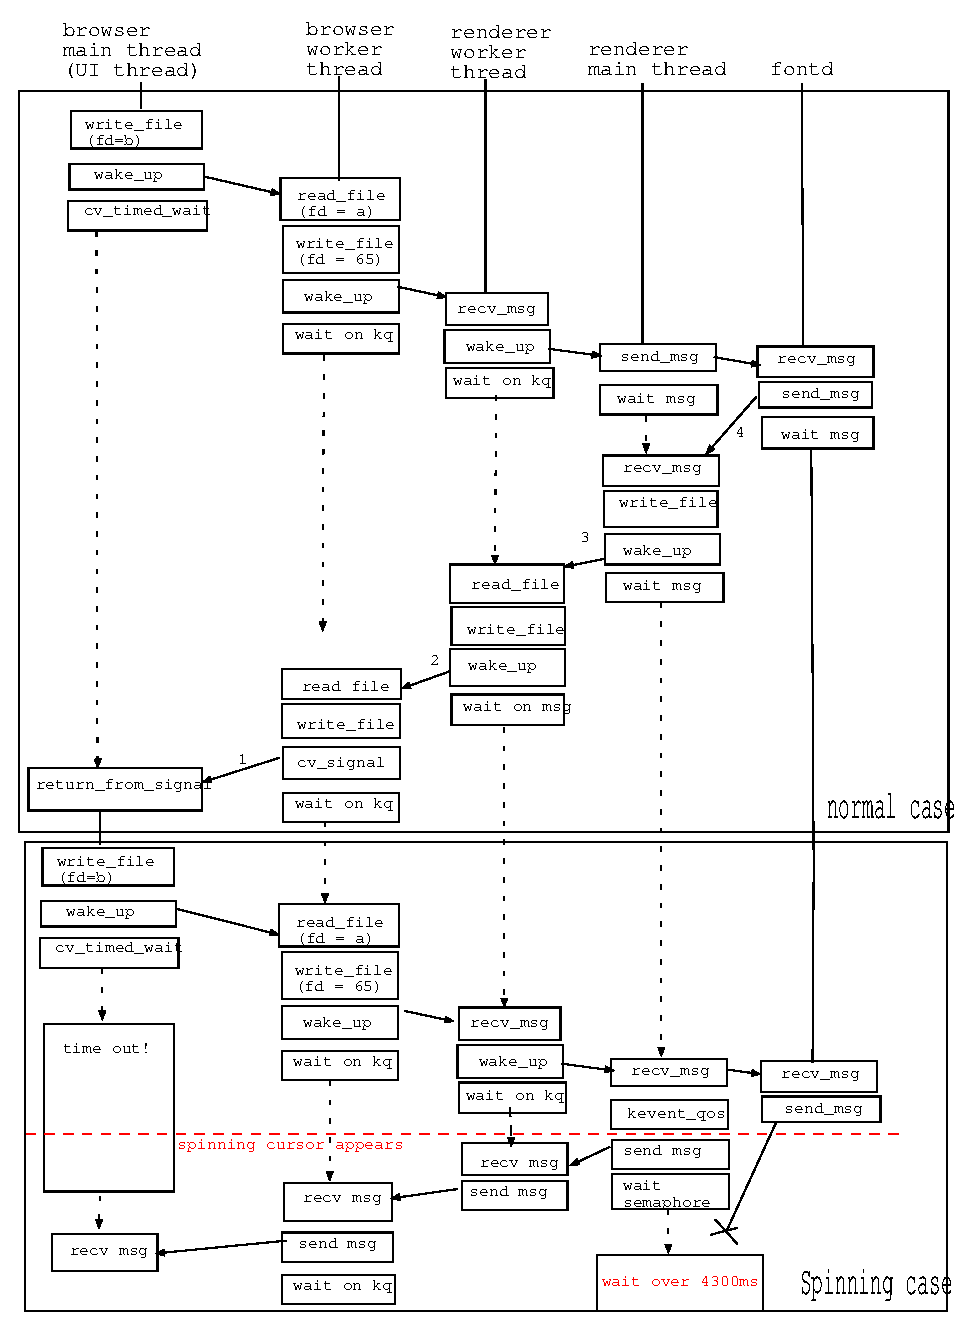
\includegraphics[width=0.8\linewidth]{chromium_case_study.eps}
    \caption{Chromium case study.}
    \label{fig:chromium-trace}
\end{figure*}

Next she ran \xxx to find the event in the main thread of the browser process.
\xxx returned a \vv{cv\_timed\_wait} event (Figure~\ref{fig:chromium-trace})
that blocked the main thread for a few seconds.  Inspection of the lightweight
call stack revealed that this wait happened within a call to
\vv{TextInputClientMac::GetFirstRectForRange}.  Without knowing the
application's semantics, she could not understand this method.  Thus she ran
\xxx to compare the spinning case to a normal case.  \xxx searched in the main
thread of the browser process for vertexes similar to this wait waiting
vertexes (contain \vv{write\_file, cv\_timed\_wait} in this case) similar to
this wait, found three, and confirmed with the user which one she wanted.

\xxx then found the normal-case wake-up path shown in the figure, which
connects five threads.  The browser main thread was signaled by a browser
worker thread as shown in step \textcircled{1} of backward slicing in Figure
\ref{fig:chromium-trace}, which in turn \vv{read\_file} in step \textcircled{2}
for IPC from a worker thread of \vv{renderer}, the daemon for rendering screens.
The \vv{renderer} worker thread is woken up by the \vv{renderer} main thread to
\vv{read\_file} \textcircled{3}, which in turn \vv{recv\_msg} \textcircled{4}
from \vv{fontd}, the font service daemon.  From this path, we could guess that
\vv{GetFirstRectForRange} was for the browser to understand the bounding box of
the search string.  \xxx further compared the wake-up path with the spinning
case, and returned the \vv{wait\_semaphore} event in the \vv{renderer} main
thread, the culprit that delayed waking up the browser main thread over 4
seconds.

What caused the wait in the \vv{renderer} main thread though?  She thus
continued diagnosis and recursively applied \xxx to the wait in \vv{renderer},
and got the wake-up path shown in the figure for this wait.  Inspection reveal
that the \vv{renderer} requested the browser's help to render Javascript and was
waiting for a reply.  At this point, a circular wait formed because the browser
was waiting for the \vv{renderer} to return the string bounding box and the
\vv{renderer} was waiting for the browser to help render Javascript.  This
circular wait was broken by a timeout in the browser main thread (the
\vv{cv\_timed\_wait} timeout was 1,500 ms).  While the system was able to make
progress, the next key press caused the spinning cursor to display for another
1,500 ms.  The timeout essentially converted a deadlock into a livelock.

\subsection{Limitations}

\xxx is designed to support interactive debugging of performance issues.  To
incrementally obtain more fine-grained event traces, it needs to rerun an
application to reproduce a performance issue.  Thus, if the issue is difficult
to reproduce, we have to rely on the log collected by the lightweight
system-wide tracing for debugging, and lose the benefits of interactivity.
Fortunately, a performance issue that almost never reproduces is probably not
as annoying as one that occurs frequently.

We implemented \xxx in the closed-source MacOS which presents a harsh test for
\xxx, but we have not ported \xxx to other operating systems yet.  It is
possible that the ideas and techniques do not generalize to other operating
systems.  However, modern operating systems share many similarities, and good
ideas tend to flow both ways, so we are hopeful that the ideas in \xxx are
generally applicable.  Similarly, the applications and performance issues used
in our evaluation may be non-representative.
